\chapter{Percettrone}
E' stato introdotto da Frank Rosenblatt, uno psicologo americano, nel 1958.



Si tratta di una semplice forma di rete neurale utilizzata per \textbf{classificare esempi linearmente separabili}.



È possibile trovare un \textbf{iperpiano} che \textbf{separi} tutti gli esempi classificati in un modo da tutti quelli classificati in un altro modo.


Un esempio:
\begin{figure}[!h]
    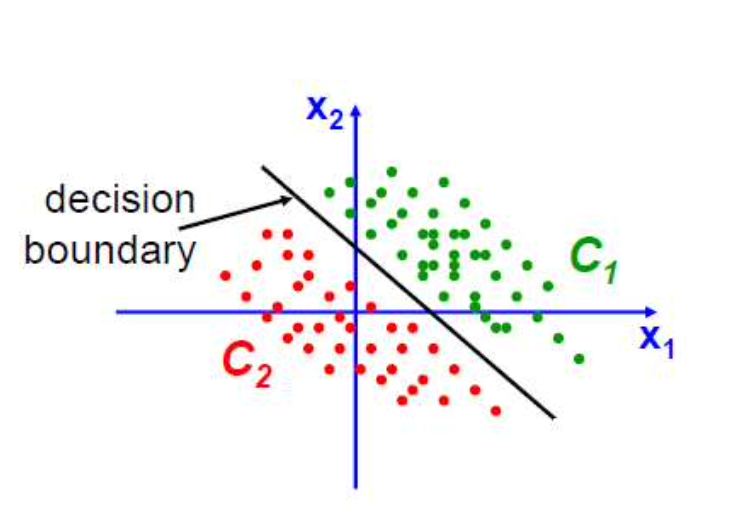
\includegraphics[scale=.5]{images/perceptron/perceptron.png}
    \centering
\end{figure}



La \textbf{struttura} del percettrone è la seguente:
\begin{itemize}
    \item \textbf{input}, il vettore \textbf{x};
    \item \textbf{output}, il vettore \textbf{y} (un singolo valore se si tratta di un neurone);
    \item \textbf{vettore dei pesi}, il vettore \textbf{w}.
\end{itemize}
\begin{figure}[!h]
    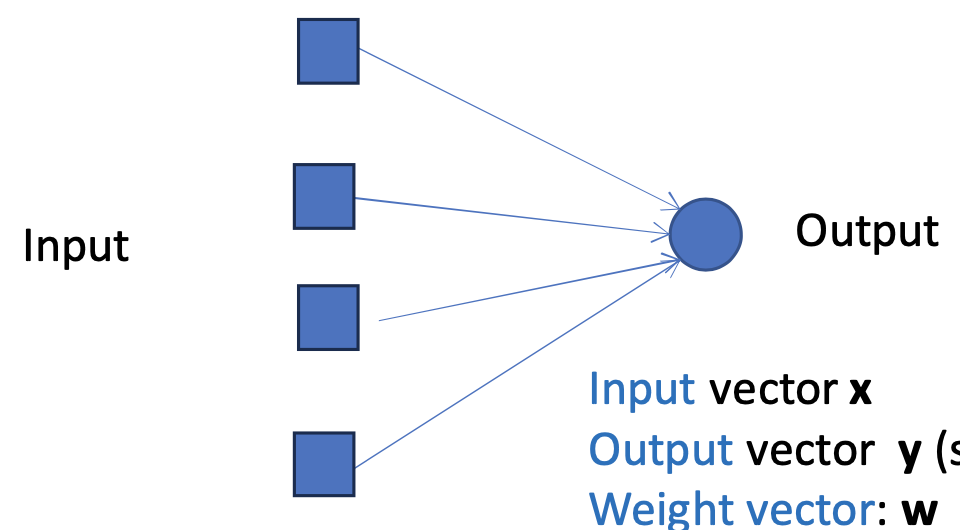
\includegraphics[scale=.5]{images/perceptron/struct.png}
    \centering
\end{figure}

Il \textbf{training set} è formato da coppie:\newline
[\textit{
(input$_1$,outputDesiderato$_1$),\newline
(input$_2$,outputDesiderato$_2$),\newline
$\dots$
}].
\newpage
\section{Principi basici delle reti neurali}
Nel cervello umano, \textbf{l'unita computazionale basica} è il \textbf{neurone}. Ci sono circa $10$ miliardi di neuroni e $60$ milioni di milioni di sinapsi.



Esattamente allo stesso modo, \textbf{anche l'unita computazionale basica delle reti neurali è il neurone}. Ed anche qui, molti neuroni sono connessi gli uni agli altri tramite le sinapsi.
\begin{figure}[!h]
    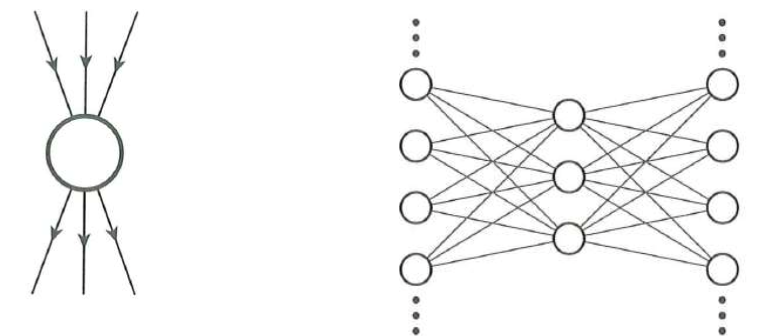
\includegraphics[scale=1]{images/perceptron/neuron01.png}
    \centering
\end{figure}



Il princpale ruolo di un neurone all'interno del cervello è quello di raccogliere, elaborare e propagare i segnali elettrici.
Il segnale elettrico in output è proporzionale al segnale in input ricevuto.



Di nuovo, esattamente allo stesso modo, \textbf{il neurone formale riceve, elabora e trasmette ai neuroni successivi l'informazione ricevuta. L'output è proporzionale all'input ricevuto}.


Le operazioni del singolo neurone \textbf{sono molto semplici}: ad esempio decidere se l'input totale è superiore o meno ad una soglia.
\begin{figure}[!h]
    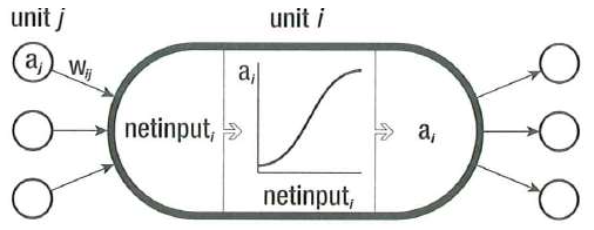
\includegraphics[scale=1]{images/perceptron/neuron02.png}
    \centering
\end{figure}
\newpage
\textbf{Neurone (McCulloch Pitts 1943)}
\begin{figure}[!h]
    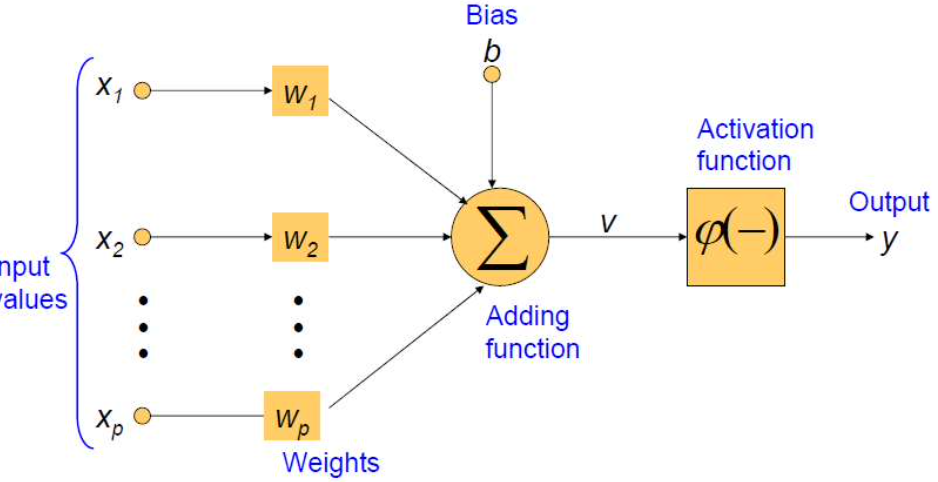
\includegraphics[scale=1]{images/perceptron/pitts.png}
    \centering
\end{figure}


\begin{itemize}
    \item vettore di input \textbf{x}
    $\begin{bmatrix}
        x_1\\
        \dots\\
        x_p
    \end{bmatrix}$;
    \item vettore dei pesi \textbf{w}
    $\begin{bmatrix}
        w_1\\
        \dots\\
        w_p
    \end{bmatrix}$.
\end{itemize}
Per ogni valore di input $x_i$, ciò che il neurone $j$ riceve è $w_{ji}x_i$. 


$w_{ji}x_i$ è il peso della sinapsi da $i$ a $j$. Così come una sinapsi può essere eccittata o inibita, così anche un peso può essere maggiore, minore o uguale a zero.
\newline
\newline
Il cosiddetto \textbf{network input} o (\textbf{netinput}) di $j=\text{\textbf{x}}\cdot\text{\textbf{w}}$ ($=\text{\textbf{x$^{\text{T}}$}}\cdot\text{\textbf{w}}=\sum_{i=1}^p\text{x}_i\text{w}_i$).
\newline
\newline
Alcune esempi di valori in input sono:
\begin{itemize}
    \item pixel values;
    \item fonemi;
    \item misurazioni;
    \item encoding di concetti di livello superiore;
    \item encoding di single parole;
    \item output di altri neuroni.
\end{itemize}
L'output del neurone dipenderà dal \textbf{netinput e dal bias}:
\begin{equation}
    y_j=\phi(u_j+b)
\end{equation}
dove $u_j+b$ rappresenta il potenziale di attivazione o campo locale di $j$.
\newpage
Tutti i neuroni hanno un \textbf{bias} che rappresenta la loro attivazione spontanea:
\begin{itemize}
    \item se bias$>0$ il neurone è spesso attivo, anche con input bassi;
    \item se bias$<0$, affinché il neurone sia attivo, i valori di input devono essere alti (rappresenta infatti una soglia).
\end{itemize}


\begin{figure}[!h]
    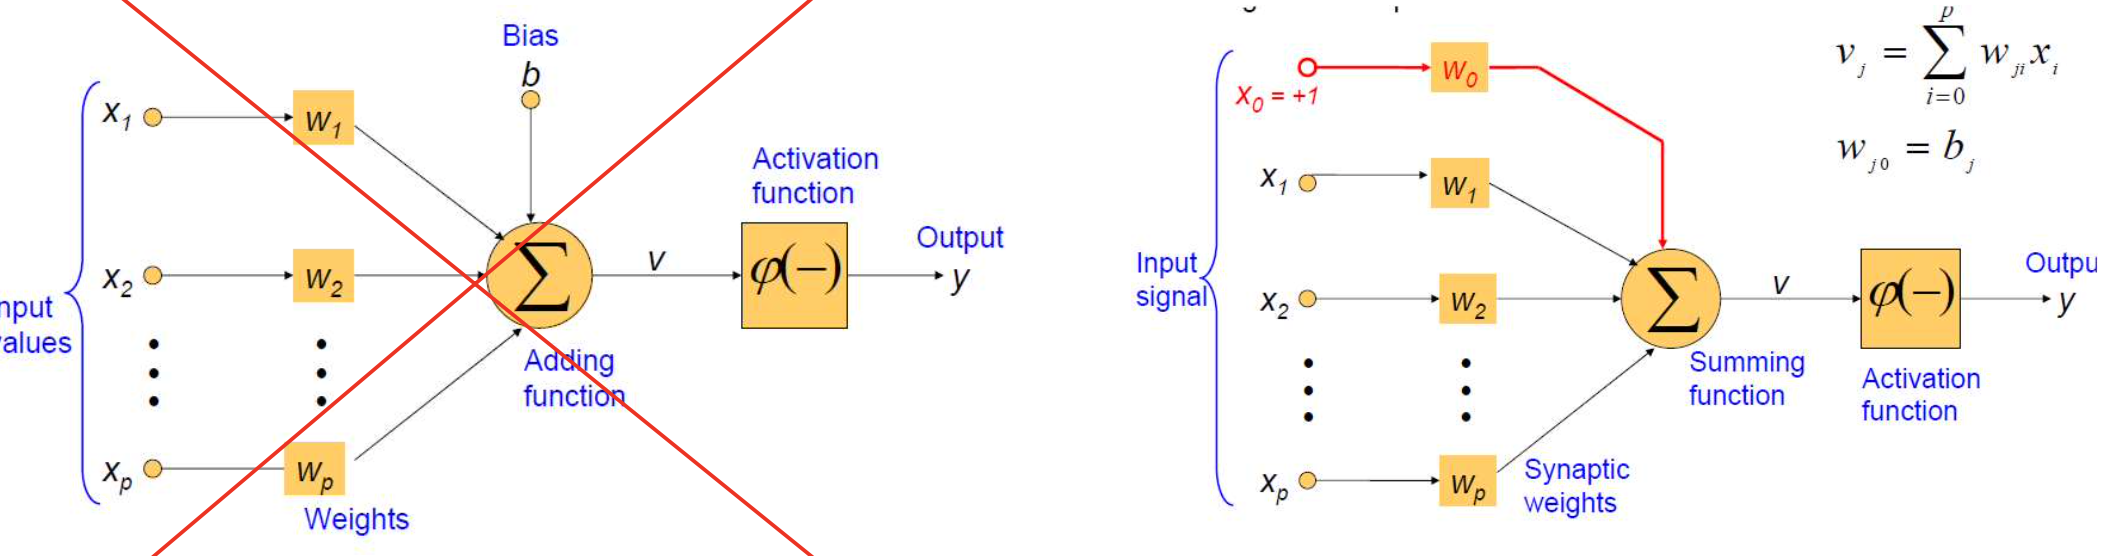
\includegraphics[scale=.4]{images/perceptron/architecture.png}
    \centering
\end{figure}


Per semplificare i calcoli, il bias del neurone $j$ può essere trattato come un elemento aggiuntivo in input  $\text{x}_0 =1$ con $\text{w}_0 =b$.
\newline
In questo caso, $\text{v}_j=\sum_{j=0}^p\text{v}_{\text{ji}}\text{x}_\text{i}$. \newline
Questa sarà l'architettura che noi utilizzeremo.\newline
\newline
\textbf{Esempio:}\newline
L'\textbf{or}, normalmente rappresentato così
\begin{gather}
    ([1,1], 1)\\
    ([1,0], 1)\\
    ([0,1], 1)\\
    ([0,0], -1)
\end{gather}
si traformerà in questo
\begin{gather}
    ([1,1,1], 1)\\ 
    ([1,1,0], 1)\\
    ([1,0,1], 1)\\
    ([1,0,0],-1).
\end{gather}
\newpage
\paragraph{La funzione di attivazione.}
Riguardo questa funzione:
\begin{itemize}
    \item l'output del percettrone sarà $1$ se $\sum_{i=0}^px_{ji}x_i>0$ (cioè se $\textbf{x}\cdot\textbf{w}>0$);
    \item l'output del percettrone sarà $-1$ se $\sum_{i=0}^px_{ji}x_i\leq0$ (cioè se $\textbf{x}\cdot\textbf{w}\leq0$).
\end{itemize}
\begin{figure}[!h]
    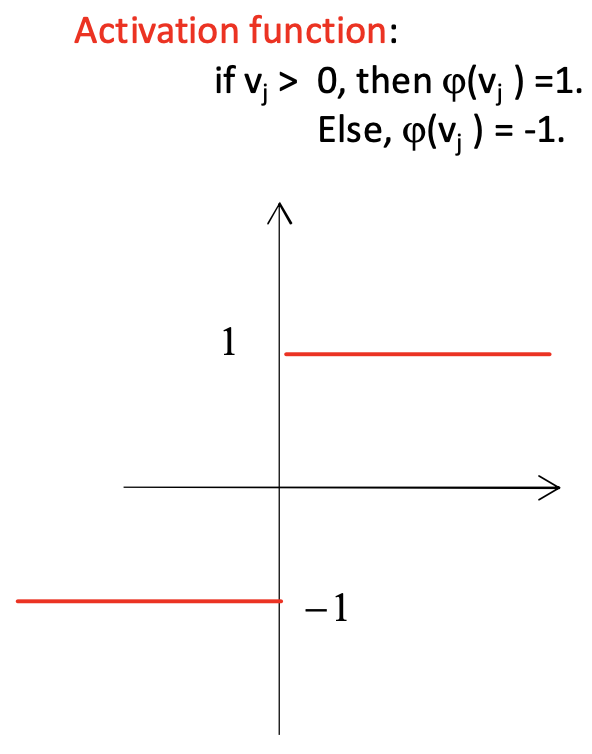
\includegraphics[scale=.4]{images/perceptron/actFun.png}
    \centering
\end{figure}


Perciò si può dire che \textbf{l'output del percettrone per un dati input dipende dal vettore dei pesi}. Infatti, data una certa configurazione \textbf{w}:
\begin{itemize}
    \item l'output sarà $1$ per tutti i vettori di input \textbf{x} tali che $\textbf{x}\cdot\textbf{w}>0$;
    \item l'output sarà $-1$ per tutti i vettori di input \textbf{x} tali che $\textbf{x}\cdot\textbf{w}\leq0$.
\end{itemize}
\begin{figure}[!h]
    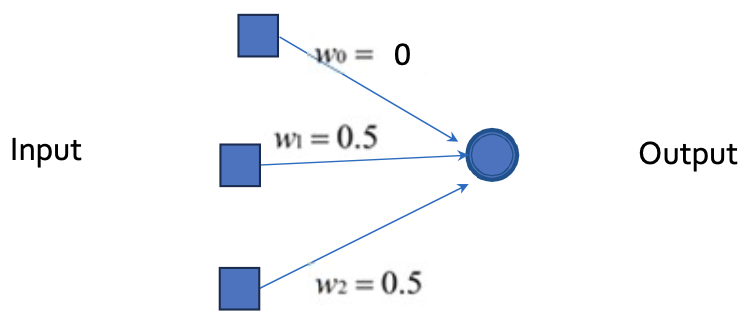
\includegraphics[scale=.8]{images/perceptron/weight.png}
    \centering
\end{figure}


Il \textbf{decision boundary} è dato da tutti gli \textbf{x} tali che $\textbf{x}\cdot\text{w}=0$.
\newline
\newline
Un esempio di una possibile soluzione per l'or è dato da $\textbf{w}_1=\textbf{w}_2=0.5$,$\textbf{w}_0=0$
\begin{figure}[!h]
    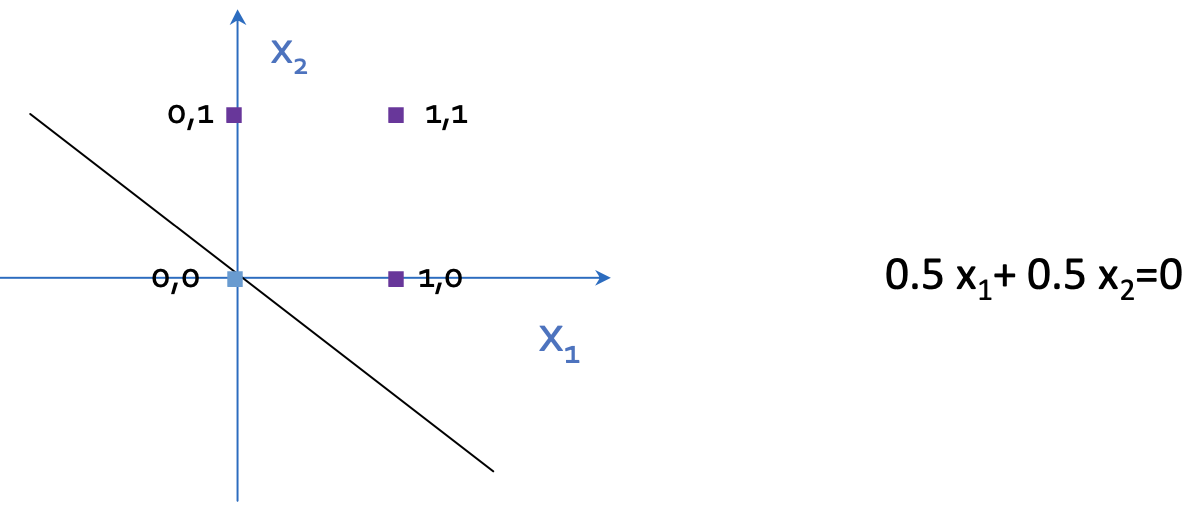
\includegraphics[scale=.5]{images/perceptron/orSolution.png}
    \centering
\end{figure}
\newpage
Il \textbf{percettrone} impara a classificare gli esempi \textbf{linearmente separabili} regolando i pesi. Gli esempi sono coppie (\textit{input, output desiderato}) che costituiscono il \textbf{training set}. Gli esempi (anche detti \textbf{pattern}) si trovano all'interno del training set. Nelle reti più complesse può essere utilizzato anche un \textbf{test set} per testare l'apprendimento della rete su un set di esempi diversi da quelli presenti nel training set.
\section{Learning Algorithm}
Il modo con cui il percettrone ottiene l'output desiderato è \textbf{modificando i pesi}. Questa modifica è ottenuta grazie all'applicazione di un algoritmo di learning basato, per esempio, \textbf{sulla correzione degli errori}. Segue la regola per la correzione dei pesi dell'$n$-esima iterazione:
\begin{itemize}
    \item $w(n+1) = w(n)$ se l'output è corretto;
    \item se l'output non è corretto:
    \begin{itemize}
        \item se l'output è minore del previsto\newline $w(n+1) = w(n) - \eta(n)x(n)$ se $x(n) \cdot w(n) > 0$ e $x(n) \in C2$;
        \item se l'output è maggiore del previsto\newline $w(n+1) = w(n) +\eta(n)x(n)$ se $x(n) \cdot w(n) \leq 0$ e $x(n) \in C1$.
    \end{itemize}
\end{itemize}
L'algoritmo continua finché ci sono elementi non classificati correttamente.\newline
%psudocodice%
Un'\textbf{epoca} è un'iterazione su tutti gli elementi del set di addestramento. Qui l'aggiornamento del peso avviene \textbf{pattern-by-pattern}: i pesi vengono aggiornati per ogni patterb classificato erroneamente.
\newline
L'algoritmo può anche essere semplificato in questo modo:
%pseudo algoritmo semplificato%
\newpage
\section{Teorema della convergenza}
Se esiste una soluzione (ovvero se il problema è linearmente separabile), l'algoritmo la trova. \newline
Ad ogni iterazione viene modificato il vettore dei pesi e, di conseguenza, il decision boundary. Il \textbf{Teorema della Convergenza garantisce che l’aggiustamento del peso termina}.
\begin{itemize}
    \item $\|w(k+1)\|^2\geq \frac{k^2\alpha^2}{\|w^*\|^2}$ (A) lower bound;
    \item $\|w(k+1)\|^2\leq k^2\beta^2$ (A) upper bound.
\end{itemize}
(A) e (B) sono compatibili se e solo se:
\begin{equation}
    \frac{k^2\alpha^2}{\|w^*\|^2}\leq k\beta,
\end{equation}
cioè
\begin{equation}
    k\leq \frac{\beta\|w^*\|^2}{\alpha^2}.
\end{equation}
\begin{figure}[!h]
    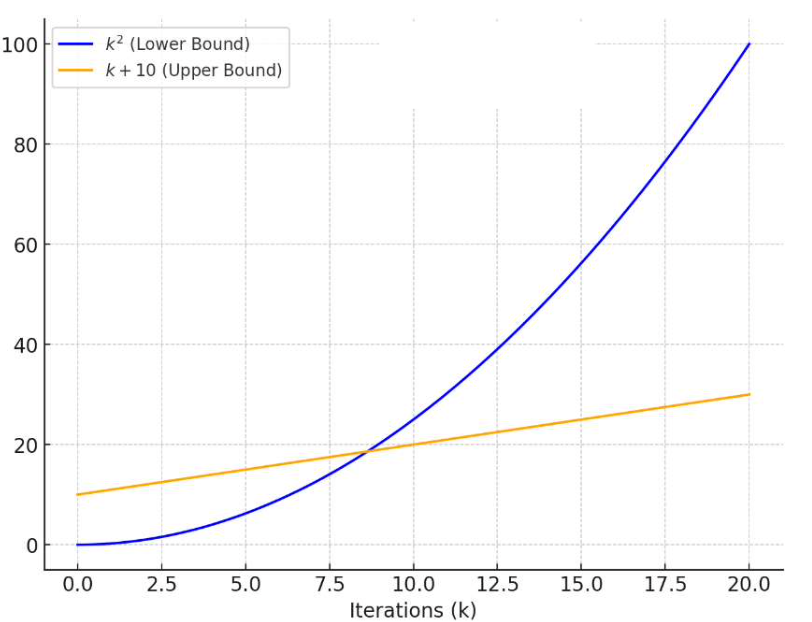
\includegraphics[scale=.8]{images/perceptron/convTheorem.png}
    \centering
\end{figure}
\newpage
\section{I limiti del percettrone e le Multilayer Networks}
Come precedentemente descritto e provato, il percettrone risolve problemi linearmente separabili come AND e OR. Ma come si comporta con i problemi che \textbf{non sono linearmente separabili} come, ad esempio, \textbf{lo XOR}?
\begin{figure}[!h]
    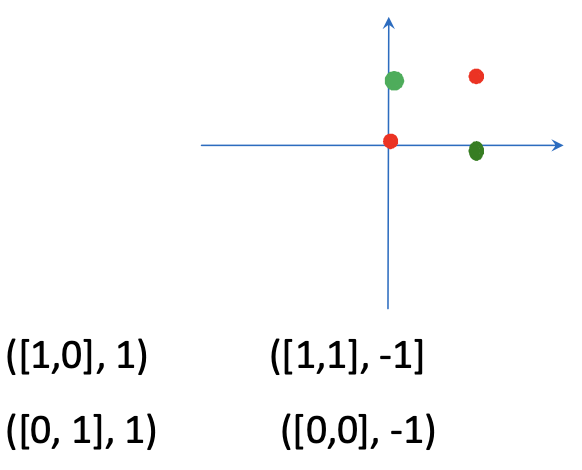
\includegraphics[scale=.8]{images/perceptron/xor.png}
    \centering
\end{figure}



Fondamentalmente, il percettrone non riesce e non può risolvere problemi di questo tipo. E la causa di ciò è proprio la natura di questi problemi, cioè il fatto che sia impossibile costruire una retta (piano, iperpiano ecc.) che separi perfettamente gli esempi del training set.\newline
Per risolverli bisogna introdurre i cosiddeti \textbf{hidden layer}, ognuno di quali risolve una parte del problema. Alla fine, si ha la costruzione della soluzione.
\begin{figure}[!h]
    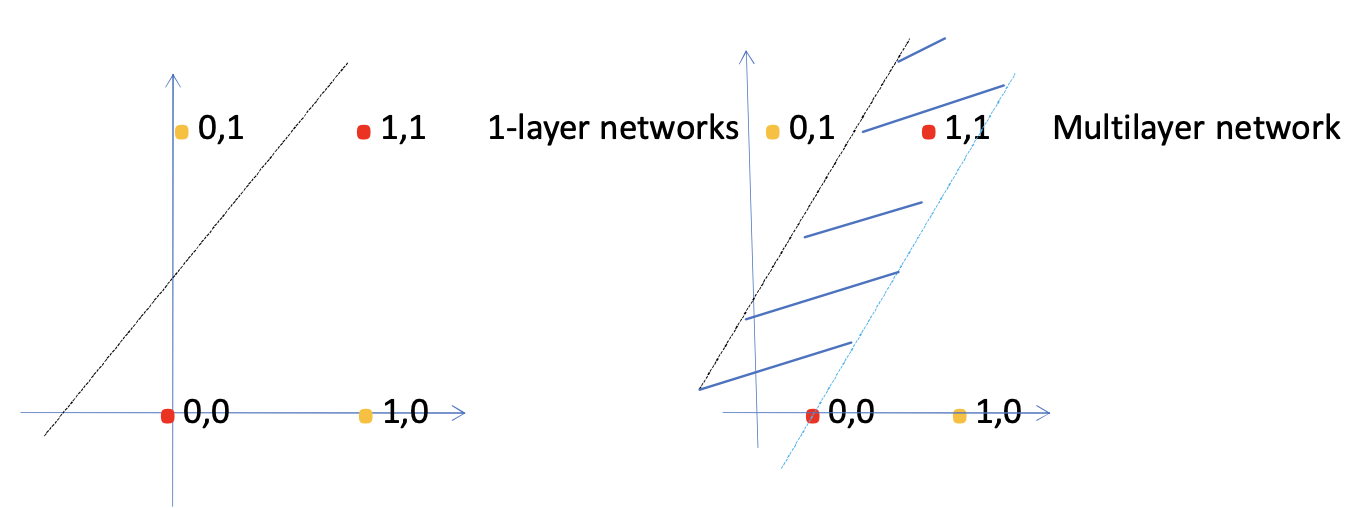
\includegraphics[scale=.75]{images/perceptron/multilayerNet.png}
    \centering
\end{figure}
\newpage

